\documentclass[a4paper, english]{article}
\usepackage{xnpig}
\usepackage{babel}
\usepackage[T1]{fontenc}
\usepackage[utf8]{inputenc}
\usepackage{acronym}
\usepackage{amsmath}
\usepackage{amssymb}
\usepackage[small,labelsep=period]{caption}
\usepackage[detect-all]{siunitx}
\usepackage{graphicx}  %figures
\usepackage{authblk}
\usepackage{booktabs}
\usepackage[total={17.15cm,22.23cm}]{geometry}
\usepackage{multicol}
\usepackage{titlesec}
\titleformat*{\section}{\normalsize\bfseries}
\usepackage[
    backend=biber,
    sorting=none,
    doi=false,
    url=false,
    isbn=false
]{biblatex}
\renewbibmacro{in:}{}
\DeclareFieldFormat*{volume}{\mkbibbold{#1}}
\addbibresource{library.bib}

\newenvironment{multicolfigure}
  {\par\medskip\noindent\minipage{\linewidth}}
  {\endminipage\par\medskip}

\DeclareCaptionLabelFormat{xnpig}{#2}
\captionsetup[figure]{labelformat=xnpig}%

\begin{document}
\title{Dark field and transmission in the Compton regime}
\author[1,2]{M. Abis}
\author[1,2]{M. Stampanoni}
\affil[1]{Paul Scherrer Institute, Villigen PSI, Switzerland}
\affil[2]{Institute for Biomedical Engineering, Swiss Federal Institute of Technology, Zurich, Switzerland}
\date{}

\maketitle
\thispagestyle{empty}
\begin{multicols}{2}
    \section{Methods}
    Three images can be simultaneously retrieved with Talbot-Lau grating interferometry.
    Besides the conventional absorption image, a phase shift~\supercite{David2002}
    and a scattering~\supercite{Pfeiffer2006} signal
    are reconstructed from the interference pattern.
    %This approach does not rely on a highly coherent source and it can be applied
    %to ordinary X-ray sources outside synchrotron facilities.

    As the design energy~$\mathcal{E}$ of the interferometer
    increases, the thickness~$h$ of the absorption gratings increases
    proportionally to~$\mathcal{E}^3$, in order to efficiently block the
    incoming radiation. Moreover, the pitch~$p$ of the grating decreases
    as~$p \propto 1/\sqrt{\mathcal{E}}$ for a constant sensitivity of the
    interferometer. The aspect ratio $2h / p \propto \mathcal{E}^{7/2}$
    increases very quickly with energy, to the point where it is impossible
    to manufacture these gratings with the currently available
    microfabrication techniques.

    In the edge-on~\supercite{david2014method} configuration
    (figure~\ref{schematic}), the gratings are illuminated from one side, so
    that the light travels through the long side of the grating. A high
    aspect ratio is achieved at the cost of the vertical spatial direction.
    A tungsten anode tube \textsc{MXR-160HP/11} is used for the experiments
    with an acceleration voltage of~\SI{160}{\kilo\volt} and a current
    of~\SI{10}{\milli\ampere}. 
    \begin{multicolfigure}
        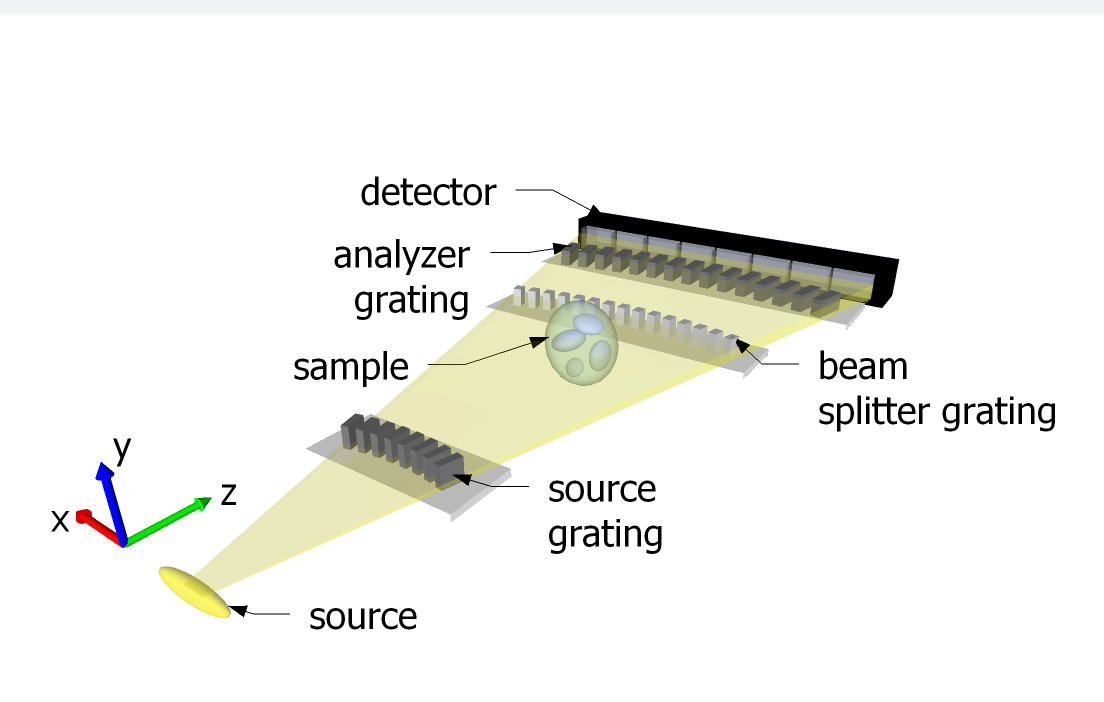
\includegraphics[width=.95\columnwidth]{figures/hDPC_setup.png}
        \captionof{figure}{Schematic of an edge-on grating
        interferometer.}\label{schematic} \end{multicolfigure}

    \section{Results}
    The experiments aims to investigate the relationship between dark field
    and absorption contrasts on different grating interferometers with a
    design energy of \SI{60}{\kilo\eV}, \SI{100}{\kilo\eV} and
    \SI{120}{\kilo\eV}. Preliminary results (figure~\ref{logratio}) show
    that the ratio $R$ is mostly independent of
    the thickness and material of the sample:
    \begin{equation*}
        R = \frac{\log\text{dark field}}{\log\text{transmission}}
    \end{equation*}
    \begin{multicolfigure}
    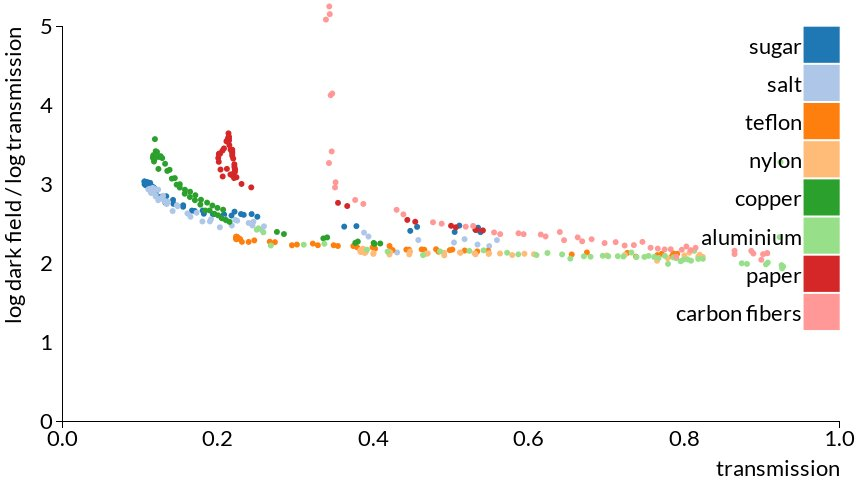
\includegraphics[width=.95\columnwidth]{figures/logratio.jpg}
        \captionof{figure}{Data recorded with a
            \SI{120}{\kilo\eV} interferometer. Different colors
    indicate different materials, while each dot represents a different
thickness.}\label{logratio}
    \end{multicolfigure}
    Lower energy interferometers have a radically different
    behaviour~\supercite{Wang2014}, and
    this typical value is then critical for the performance of the
    interferometer. As the value $R$ increases, the phase stepping curves
    reach zero visibility for weaker absorbing samples. In such conditions,
    the differential phase cannot be retrieved.

    \section{Acknowledgements}
    This work has been partially by the ERC Grant ERC-2012-StG 310005-PhaseX.
    \printbibliography{}

\end{multicols}
\end{document}
